%%%%%%%%%%%%%%%%%%%%%%%%%%%%%%%%%%%%%%%%%
% Arsclassica Article
% LaTeX Template
% Version 1.1 (1/8/17)
%
% This template has been downloaded from:
% http://www.LaTeXTemplates.com
%
% Original author:
% Lorenzo Pantieri (http://www.lorenzopantieri.net) with extensive modifications by:
% Vel (vel@latextemplates.com)
%
% License:
% CC BY-NC-SA 3.0 (http://creativecommons.org/licenses/by-nc-sa/3.0/)
%
%%%%%%%%%%%%%%%%%%%%%%%%%%%%%%%%%%%%%%%%%

%----------------------------------------------------------------------------------------
%	PACKAGES AND OTHER DOCUMENT CONFIGURATIONS
%----------------------------------------------------------------------------------------

\documentclass[
10pt, % Main document font size
a4paper, % Paper type, use 'letterpaper' for US Letter paper
oneside, % One page layout (no page indentation)
%twoside, % Two page layout (page indentation for binding and different headers)
headinclude,footinclude, % Extra spacing for the header and footer
BCOR5mm, % Binding correction
]{scrartcl}

% \usepackage{blindtext}
% \usepackage{quotchap}
\usepackage{float}
\usepackage{hyperref}
\usepackage{nicematrix}
\usepackage[T1]{fontenc}
\usepackage[scaled=0.85]{beramono}
\usepackage{xcolor}
\definecolor{mygray}{gray}{0.9}
\usepackage{fvextra}
\usepackage{amsmath}
\usepackage{amsthm}
\usepackage{physics}
\usepackage{tcolorbox}
\usepackage{graphicx, wrapfig, lipsum}

\newenvironment{code}%
 {\VerbatimEnvironment
  \begin{tcolorbox}[colback=mygray, boxsep=0pt, arc=0pt, boxrule=0pt]
  \begin{Verbatim}[fontsize=\scriptsize, commandchars=\\\{\},
    breaklines, breakafter=*, breaksymbolsep=0.5em,
    breakaftersymbolpre={\,\tiny\ensuremath{\rfloor}}]}%
 {\end{Verbatim}%
  \end{tcolorbox}}


%%%%%%%%%%%%%%%%%%%%%%%%%%%%%%%%%%%%%%%%%
% Arsclassica Article
% Structure Specification File
%
% This file has been downloaded from:
% http://www.LaTeXTemplates.com
%
% Original author:
% Lorenzo Pantieri (http://www.lorenzopantieri.net) with extensive modifications by:
% Vel (vel@latextemplates.com)
%
% License:
% CC BY-NC-SA 3.0 (http://creativecommons.org/licenses/by-nc-sa/3.0/)
%
%%%%%%%%%%%%%%%%%%%%%%%%%%%%%%%%%%%%%%%%%

%----------------------------------------------------------------------------------------
%	REQUIRED PACKAGES
%----------------------------------------------------------------------------------------

\usepackage[
nochapters, % Turn off chapters since this is an article        
beramono, % Use the Bera Mono font for monospaced text (\texttt)
eulermath,% Use the Euler font for mathematics
pdfspacing, % Makes use of pdftex’ letter spacing capabilities via the microtype package
dottedtoc % Dotted lines leading to the page numbers in the table of contents
]{classicthesis} % The layout is based on the Classic Thesis style

% \usepackage{blindtext}
% \usepackage{quotchap}
\usepackage{arsclassica} % Modifies the Classic Thesis package


\usepackage{epigraph}

% \epigraphsize{\small}% Default
\setlength\epigraphwidth{8cm}
\setlength\epigraphrule{0pt}

\usepackage{etoolbox}

\makeatletter
\patchcmd{\epigraph}{\@epitext{#1}}{\itshape\@epitext{#1}}{}{}
\makeatother

\usepackage[T1]{fontenc} % Use 8-bit encoding that has 256 glyphs

\usepackage[utf8]{inputenc} % Required for including letters with accents

\usepackage{graphicx} % Required for including images
\graphicspath{{Figures/}} % Set the default folder for images

\usepackage{enumitem} % Required for manipulating the whitespace between and within lists

\usepackage{lipsum} % Used for inserting dummy 'Lorem ipsum' text into the template

\usepackage{subfig} % Required for creating figures with multiple parts (subfigures)

\usepackage{amsmath,amssymb,amsthm} % For including math equations, theorems, symbols, etc

\usepackage{varioref} % More descriptive referencing

%----------------------------------------------------------------------------------------
%	THEOREM STYLES
%---------------------------------------------------------------------------------------

\theoremstyle{definition} % Define theorem styles here based on the definition style (used for definitions and examples)
\newtheorem{definition}{Definition}

\theoremstyle{plain} % Define theorem styles here based on the plain style (used for theorems, lemmas, propositions)
\newtheorem{theorem}{Theorem}

\theoremstyle{remark} % Define theorem styles here based on the remark style (used for remarks and notes)

%----------------------------------------------------------------------------------------
%	HYPERLINKS
%---------------------------------------------------------------------------------------

\hypersetup{
%draft, % Uncomment to remove all links (useful for printing in black and white)
colorlinks=true, breaklinks=true, bookmarks=true,bookmarksnumbered,
urlcolor=webbrown, linkcolor=RoyalBlue, citecolor=webgreen, % Link colors
pdftitle={}, % PDF title
pdfauthor={\textcopyright}, % PDF Author
pdfsubject={}, % PDF Subject
pdfkeywords={}, % PDF Keywords
pdfcreator={pdfLaTeX}, % PDF Creator
pdfproducer={LaTeX with hyperref and ClassicThesis} % PDF producer
} % Include the structure.tex file which specified the document structure and layout

\hyphenation{Fortran hy-phen-ation} % Specify custom hyphenation points in words with dashes where you would like hyphenation to occur, or alternatively, don't put any dashes in a word to stop hyphenation altogether

%----------------------------------------------------------------------------------------
%	TITLE AND AUTHOR(S)
%----------------------------------------------------------------------------------------

\title{\normalfont{\spacedallcaps{Jogging a Hamiltonian}:\\ \LARGE{Simulating Hamiltonians with Quantum Walks and other methods}}} % The article title

%\subtitle{Subtitle} % Uncomment to display a subtitle

\author{\spacedlowsmallcaps{Rutvij \textsuperscript{1}  and Arjo \textsuperscript{2}}} % The article author(s) - author affiliations need to be specified in the AUTHOR AFFILIATIONS block

\date{Apr 28, 2022} % An optional date to appear under the author(s)

%----------------------------------------------------------------------------------------

\begin{document}

%----------------------------------------------------------------------------------------
%	HEADERS
%----------------------------------------------------------------------------------------

\renewcommand{\sectionmark}[1]{\markright{\spacedlowsmallcaps{#1}}} % The header for all pages (oneside) or for even pages (twoside)
%\renewcommand{\subsectionmark}[1]{\markright{\thesubsection~#1}} % Uncomment when using the twoside option - this modifies the header on odd pages
\lehead{\mbox{\llap{\small\thepage\kern1em\color{halfgray} \vline}\color{halfgray}\hspace{0.5em}\rightmark\hfil}} % The header style

\pagestyle{scrheadings} % Enable the headers specified in this block

%----------------------------------------------------------------------------------------
%	TABLE OF CONTENTS & LISTS OF FIGURES AND TABLES
%----------------------------------------------------------------------------------------

\maketitle % Print the title/author/date block

\setcounter{tocdepth}{2} % Set the depth of the table of contents to show sections and subsections only


\let\thefootnote\relax\footnotetext{\textsuperscript{1} \textit{Rutvij Menavlikar}, CQST, IIITH\\ \textsuperscript{2}  \textit{Alapan Chaudhuri}, CQST, IIITH}

\begin{figure}[H]
    \centering
    
\includegraphics[width=60mm]{images/IIIT_Hyderabad_Logo.jpg}
\end{figure}

\tableofcontents

\section*{Abstract}
The problem of efficiently simulating a Hamiltonian is one of the long standing problems in computational physics. Today, the problem of Hamiltonian simulation stands as one of the most impacting and significant contribution of quantum computers. Furthermore since it is a BQP-complete problem, devising any efficient classical algorithm for the same is believed to be intractable.\newline

In this project, we plan to study and analyse Hamiltoninan simulation using quantum walks. We will also compare the efficiency of these algorithms with other methods such as trotterization and quantum signal processing.

% \tableofcontents % Print the table of contents
% \vfill
% \hspace{0pt}
% \pagebreak

\section{Introduction}
Hamiltonian simulation serves as the basis for many problems in science. The universe is of quantum nature, which means that to simulate particles or any other natural entities you need to simulate its Hamiltonian. However, computing the evolution given the Hamiltonian is also not very straightforward.\newline

Due to the discrete nature of classical computers, it is not possible to efficiently simulate any of the above on the same. This gives quantum computers an edge since they can work with qubits to simulate the dynamics of a system given its Hamiltonian. This makes Hamiltonian Simulation the most impacting and significant contribution of quantum computers.\newline

Furthermore, simulating hamiltonian is a $BQP$-complete problem. Thus, it is believed to be intractable by classical computers. Devising any efficient classical algorithm for hamiltonian simulation would mean proving that $P = BQP$.

\subsection{Why simulate Hamiltonians?}
Computational simulation of the physical systems provides important insights and acts as a bridge between theory and experiments.\newline

Moreover, it has more than a handful of applications, namely:
\begin{itemize}
    \item Drug design and protein folding: Finding the native structure of the protein is equivalent to the problem of finding the ground state of the system.
    \item Graph theoretic problems: Several graph theory related problems such as Graph Coloring (which is NP-complete) can be cleverly mapped to finding ground states of some classes of Hamiltonians.
    \item Note that finding the ground state of an Hamiltonian is equivalent to finding the $\min \bra{\phi}H\ket{\phi}, \forall\ \ket{\phi}$.
    \item Furthermore, Hamiltonian simulation can be used as a subroutine for implementing continuous-time quantum walks and solving linear equations, amongst others.
\end{itemize}

\subsection{Why simulate Hamiltonians in quantum computers?}
Computational simulation of the physical systems provides important insights and acts as a bridge between theory and experiments. But can a quantum system be efficiently simulated by a classical computer? The answer is certainly (almost), ‘No!’ as said by Bell. Even simulation using pseudo-random variables has exponential computational overhead.\newline

In the case where the Hamiltonian consists of a sum of interaction terms between small subsystems, the simulation is thought to be exponentially more efficient than classical simulation.

\section{The Hamiltonian}
A Hamiltonian can be time-independent (then you are lucky) or time-dependent.
\begin{itemize}
    \item Time-independent: $U(t) = e^{-iHt}$
    \item Time-dependent: $U(t) = e^{-i \int_0^t H(s) \ds}$
\end{itemize}
\subsection{Local Hamiltonians}
$$H = \sum_{j = 1}^n H_j$$
Here, $H$ denotes a local hamiltonian where each $H_j$ acts on $k = O(1)$ qubits.

\subsection{Sparse Hamiltonians}
Consider the matrix form of the Hamiltonian, $H$, to be $N\times N$. Then, $H$ is said to be sparse if it has at most $d$ non zero entries per row $d = \text{poly}(\log N)$. Some interesting points on sparse Hamiltonians:
\begin{itemize}
    \item There should exist some way for efficiently computing the location and value of the $j^\text{th}$ nonzero entry $\forall\ r \in$ rows of $H$. This is called row computability.
    \item A $k$-local Hamiltonian with $n$ terms is $d$-sparse with $d = 2^k n$.
    \item A $k$-local Hamiltonian with $n$ terms can be expressed as a linear combination of $\leq n4^k$ Pauli operators, each of which are unitaries.
\end{itemize}

\subsection{Problem of efficient decomposition}
Finding the efficient decomposition of a given Hamiltonian is not an easy task. One approach for dealing with the same for a sparse Hamiltonian ($H$) is by representing $H$ in terms of a graph and having its edges colored. Now, given that a sparse graph can be efficiently colored using only local information, we can conclude that this procedure will result in a decomposition yielding efficient simulations. In layman terms, the simulation breaks into small pieces that are easy to handle (shown below diagramatically).
\begin{figure}[H]
    \centering
    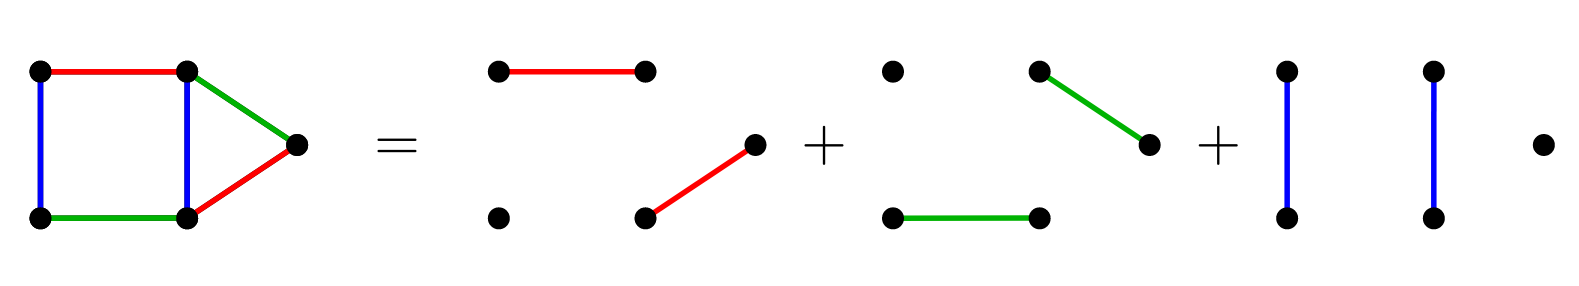
\includegraphics[width=\linewidth]{images/sparse_graph.png}
    % \caption{Capt}
    % \label{fig:my_label}
\end{figure}

\begin{figure}[H]
    \centering
    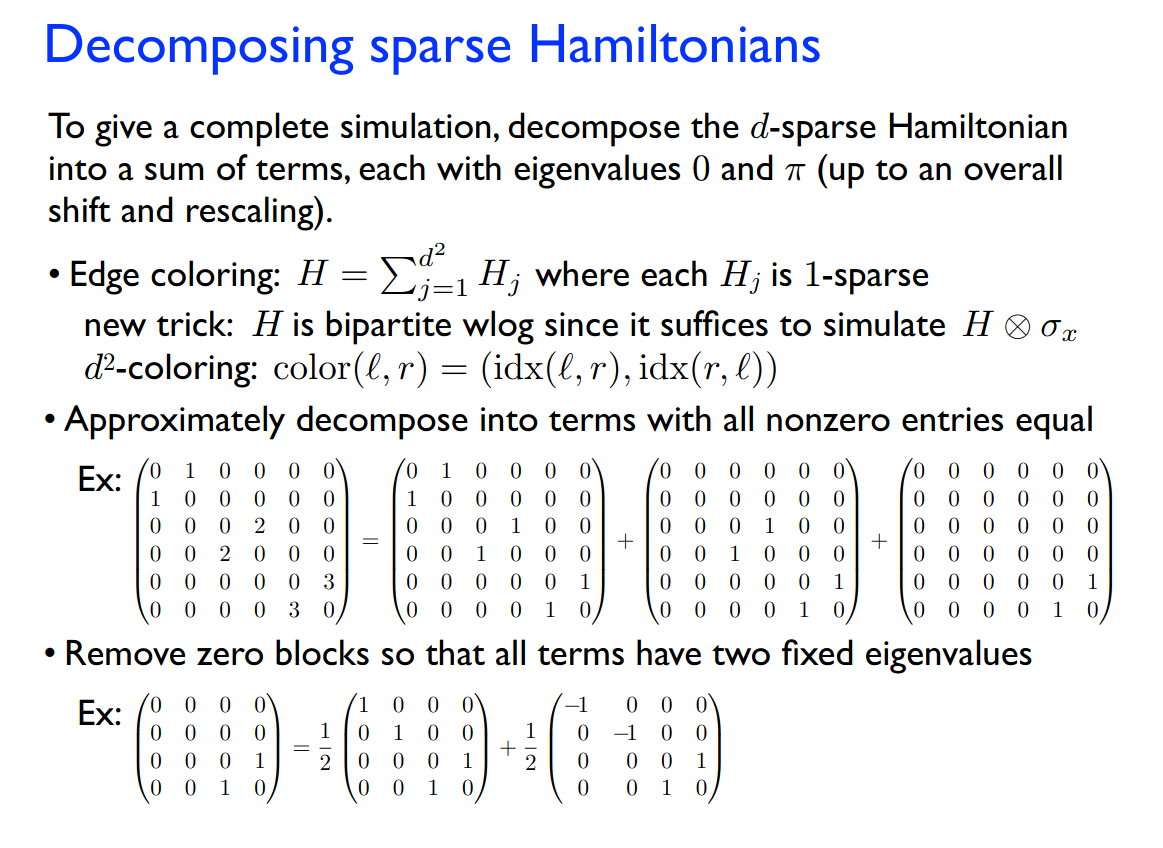
\includegraphics[width=\linewidth]{decompose.png}
    \caption{Example decomposition of sparse Hamiltonians}
    % \label{fig:my_label}
\end{figure}
\section{Algorithms for sparse Hamiltonian simulation}
Today, there exists several frameworks for simulating Hamiltonians, namely:
\begin{itemize}
    \item \textbf{Trotterization}: This was described by Zeeshan, Shreyas and Hrishi, in quite some detail.
    \item \textbf{Truncated Taylor Series}: We shall describe this algorithm in some depth, before moving on with quantum walks.
    \item \textbf{Quantum Walks}: The main focus of our project which we describe below in quite some detail. 
    \item \textbf{Quantum Signal Processing}: This procedure gives us the best known theoretical bounds through a framework called qubitization.
\end{itemize}

Now, for implementation purposes over near term NISQ models of quantum computation, Trotterization appears to be the way to go, even though it is theoretically slower with respect to algorithms such as qubitization. This is because it is simpler to implement and uses way less ancilla qubits.\newline

Now, it is also worth noting that theoretically Trotterization in itself is not inefficient. On the contrary, it is quite efficient achieving a complexity only slightly superlinear in t. Why is that good? Well, because the no-fast-forwarding theorem implies that simulation in sublinear time is not possible.

\subsubsection{No-fast-forwarding Theorem}
Fast forwarding is the ability to simulate (using a quantum computer) the evolution of a given system governed by a certain Hamiltonian $H$ to within time $t$, but such that the simulation takes time which is much less than $t$.\newline

The no-fast-forwarding theorem states that fast forwarding any physically realistic Hamiltonian (which can be efficiently simulated by a quantum circuit) is highly unlikely. This is proven by showing that even for $2$-sparse row-computable Hamiltonians the possibility of exponential fast-forwarding implies $BQP = PSPACE$.

\subsection{Complexity comparision for sparse Hamiltonian simulation}
\begin{center}
\begin{tabular}{ *5l }   \toprule
\emph{Method} && \emph{Query Complexity} & \emph{Gate Complexity}  \\\midrule
Lee-Suzuki Trotter && $O\left(d^{3}t\left({\frac {dt}{\epsilon }}\right)^{{\frac {1}{2}}k}\right)$  & $O\left({\frac {t^{2}}{\epsilon }}\right)$\\ \\ 
Truncated Taylor Series && $O\left({\frac {d^{2}||H||_{max}\log {\frac {d^{2}||H||_{max}}{\epsilon }}}{\log \log {\frac {d^{2}||H||_{max}}{\epsilon }}}}\right)$ & $O\left({\frac {t\log\left({\frac {t}{\epsilon }}\right)}{\log \log {\frac {t}{\epsilon }}}}\right)$\\ \\
Quantum Walks && $O\left(d||H||_{max}{\frac {t}{\sqrt {\epsilon }}}\right)$ & $O\left({\frac {t}{\sqrt {\epsilon }}}\right)$\\ \\
Qubitisation && $O\left(td||H||_{max}+{\frac {\log {\frac {1}{\epsilon }}}{\log \log {\frac {1}{\epsilon }}}}\right)$ & $O\left(t+\log {\frac {1}{\epsilon }}\right)$\\
\bottomrule
\hline
\end{tabular}
\end{center}

\subsection{Unsolved questions}
\begin{enumerate}
    \item How well do the bounds reflect upon implementation over NISQ frameworks?
    \item Quantum walks serve as a framework for universal computation. In that case, can we leverage Hamiltonian simulation using quantum walks to solve unrelated graph theoretic and combinatorial optimization problems?
    \item The problem of efficient decomposition is required to be tackled for general cases.
    \item Given possible frameworks for Hamiltonian simulation and a given Hamiltonian with a favoured decomposition, which framework will be most suitable for simulating it? Can this problem be solved using decision trees/random forests by keeping calculating information gained about the original Hamiltonian by studying how it is deemed to affect chosen sets of qubits?
    \item How to deal with non-sparse Hamiltonians?
\end{enumerate}

\section{Truncated Taylor Series}
Any Hamiltonian can be decomposed as a linear combination of unitary matrices. Now, let $H$ be some given Hamiltonian. Then, we have the following:
\begin{itemize}
    \item $H = \sum_{j = 1}^n \alpha_j H_j$
    \item Here, each $H_j$ is unitary and a mechanism is available for implementing that unitary.
    \item Local Hamiltonians: These can be decomposed into a sum of tensor products of Pauli matrices where each term acts nontrivially on a constant number of qubits.
    \item We can use this algorithm, broadly, for all families of sparse Hamiltonians.
\end{itemize}

\subsection{The Simulation}
Consider $U(t) = e^{-iHt}$ and we wish to simulate this evolution within error $\epsilon$.
\begin{itemize}
    \item Divide the evolution time into $r$ segments.
    \item Within each segment we have $U_r = e^{-iHt/r} \approx \sum_{k = 0}^{K} \frac{1}{k!} (-iHt/r)^k$, where the Taylor series is truncated to $K$.
    \item For $U_r$, the corresponding error should be $\leq \epsilon/r$.
    \item Given, $r \geq ||H||t$, we can choose $K = O(\frac{\log(r/\epsilon)}{\log\log{(r/\epsilon)}})$.
    \item Overall complexity $\approx rK$.
\end{itemize}
\begin{align*}
U_r &= \sum_{k = 0}^K \frac{(-iHt/r)^k}{k!}\\ &= \sum_{k = 0}^K \sum_{l_1, l_2,\ldots, l_k = 1}^L \frac{(t/r)^k}{k!} \alpha_l_1,\ldots, \alpha_l_k (-i)^k H_l_1 \ldots H_l_k\\ &= \sum_{j = 0}^{J} \beta_j V_j
\end{align*}

Here, $U_r$ is a LCU of $V_j = (-i)^k H_l_1 \ldots H_l_k$ with the coefficients $\beta_j$ described above. Now, without loss of generality we can set each of $\alpha_l \geq 0 \implies \beta_j > 0$. Note that, $U_r = \Tilde{U}(t/r)$ where $\Tilde{U}$ denotes truncation.

$$||\Tilde{U(t/r)} - U(t/r)|| \leq e^{\alpha t /r} \frac{(\alpha t/r)^{K + 1}}{(K + 1)!}$$

Now, here we have the following as well.
\begin{itemize}
    \item $\alpha = \sum_l \alpha_l$
    \item Given $\epsilon$, $K = O\left(\frac{\log\frac{\alpha t}{\epsilon}}{\log\log \frac{\alpha t}{\epsilon}}\right)$
    \item Required complexity = $O(rK)$
\end{itemize}

\subsection{Implementation}
In order to be able to implement the given sum of unitary operators, we introduce a few subroutines. The first subroutine we introduce is the $\operatorname{SELECT}$ such that $\operatorname{SELECT(V)}\ket{j}\ket{\psi} = \ket{j}V_j\ket{\psi}$. Thus, $\operatorname{SELECT}$ serves as some form of reflection.\newline

Now, in order to simulate $\Tilde{U}$, we first introduce a $J + 1$ dimensional unitary $B$ to prepare the required ancillary state (where $s = \sum_{j = 0}^{J}\beta_j$).
$$B \ket{0} = \frac{1}{\sqrt s} \sum_{j = 0}^{J} \sqrt{\beta_j}\ket{j}$$

Now, let us define the operator $W = (B^{\dagger}\otimes \mathbb{I})\operatorname{SELECT}(V)(B \otimes \mathbb{I})$ then we have the following for some $\ket{\phi}$ whose ancillary state is supported in the subspace orthogonal to $\ket{0}$.

$$W\ket{0}\ket{\psi} = \frac{1}{s} \ket{0} \Tilde{U}\ket{\psi} + \sqrt{1 - \frac{1}{s^2}}\ket{\phi}\\
\implies P(W\ket{0}\ket{\psi}) = \frac{1}{s} \ket{0} \Tilde{U}\ket{\psi}$$

Here, $P$ denoted the projection operator $\ket{0}\bra{0}\otimes \mathbb{I}$. The value of $s$ can be adjusted by choosing the size of the segments. Now, using the \textit{Approximate segment lemma} and \textit{Oblivious amplitude amplification}, we obtain that if $\Tilde{U}$ is unitary then it can be implemented using $W$, $W^\dagger$ and with the $(J + 1)$-dimensional ancilla reflection $R = 1 - 2P$.\newline

To conclude, if $\Tilde{U}$ is unitary and $A = -WRW^\dagger RW$ then, $A\ket{0}\ket{\psi} = \ket{0}\Tilde{U}\ket{\psi}$.

\subsection{Possible future work}
Now, it is worth noting that in this formulation, the truncation error exists even if the Hamiltonian consists of mutually commutative terms. Thus, we can ideally come up with faster and less error prone algorithms by further exploiting commutative and anti-commutative relations.

\section{Time-dependent Hamiltonians}
We observe time dependent Hamiltonians when our system has external classical control on it. then, we can not represent the corresponding unitary evolution as a closed form expression. Thus, $U$ remains as following.

$$U(t) = e^{-i \int_0^t H(s) \ds}$$

For this time-dependent case, we do have an infinite-series representation - an analog for Taylor series in the time-independent case. This representation is called the Dyson series expression.

\subsection{Dyson expansion of $U$}
$$U(t) = 1 + (-i) \int_0^t dt_1H(t_1) + (-i)^2 \int_0^t \int_0^t_1 dt_1 dt_2 H(t_1) H(t_2) + \ldots$$

Note that, in this case ordering highly matters because when we are considering $H(t)$, it may not always commute with itself (because it is time dependent).

\begin{figure}[H]
    \centering
    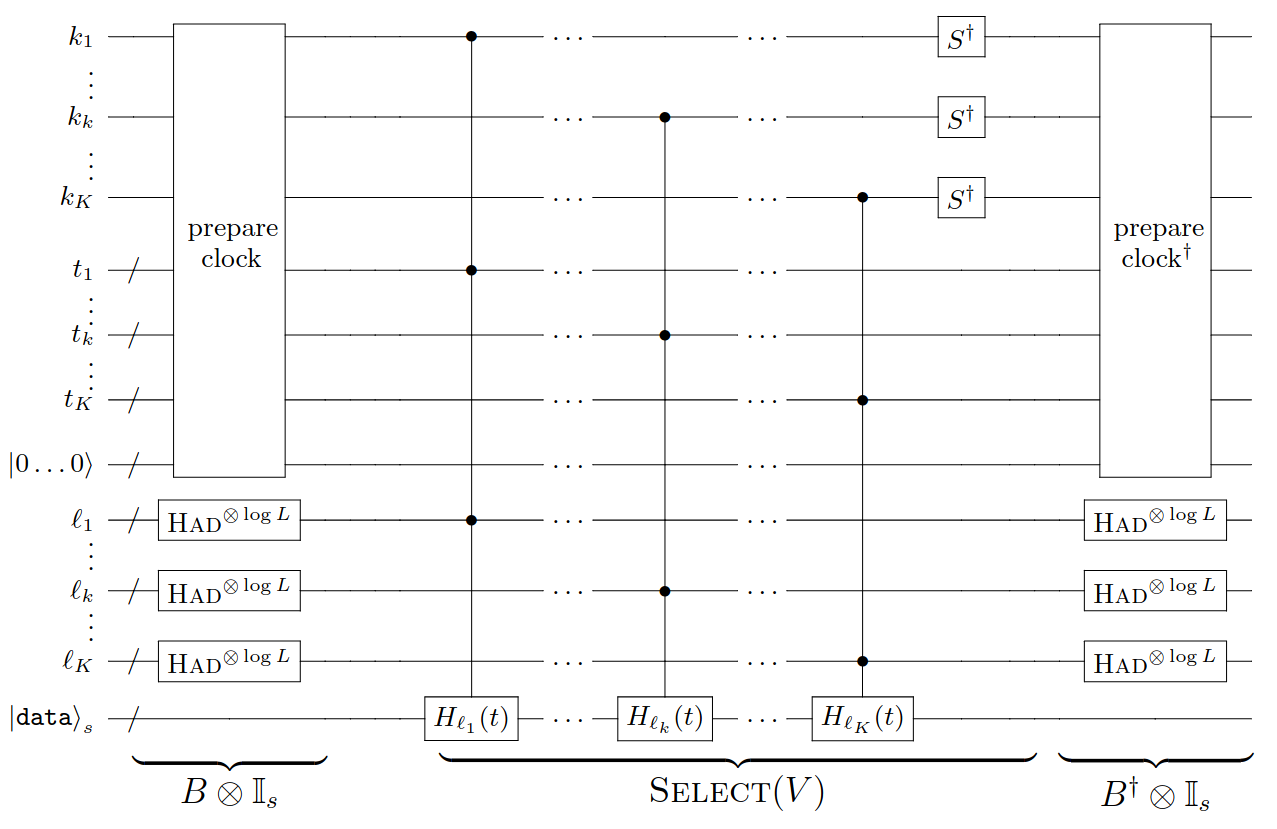
\includegraphics[width=\linewidth]{images/trunc.png}
    \caption{Truncated Dyson series implementation for time-dependent Hamiltonian simulation}
\end{figure}

\section{Quantum Walks}

Quantum walks, the quantum mechanical counterpart of classical random walks are an advanced tool for building quantum algorithms that have been recently shown to constitute a universal model of quantum computation. In contrast to the classical random walk, where the walker occupies definite states and the randomness arises due to stochastic transitions between states, in quantum walks randomness arises through:
\begin{enumerate}
    \item Quantum superposition of states,
    \item Non-random, reversible unitary evolution
    \item Collapse of the wave function due to state measurements.
\end{enumerate}

The quantum dynamics of any discrete system can be captured by a quantum walk on a network, which is a universal model for quantum computation. Besides being a useful primitive to design quantum algorithms, quantum walks are a powerful tool to model transport in quantum systems such as the transfer of excitations in light-harvesting systems. Studying the long-time dynamics of quantum walks on networks is crucial to the understanding of these diverse problems.

\begin{figure}[H]
    \centering
    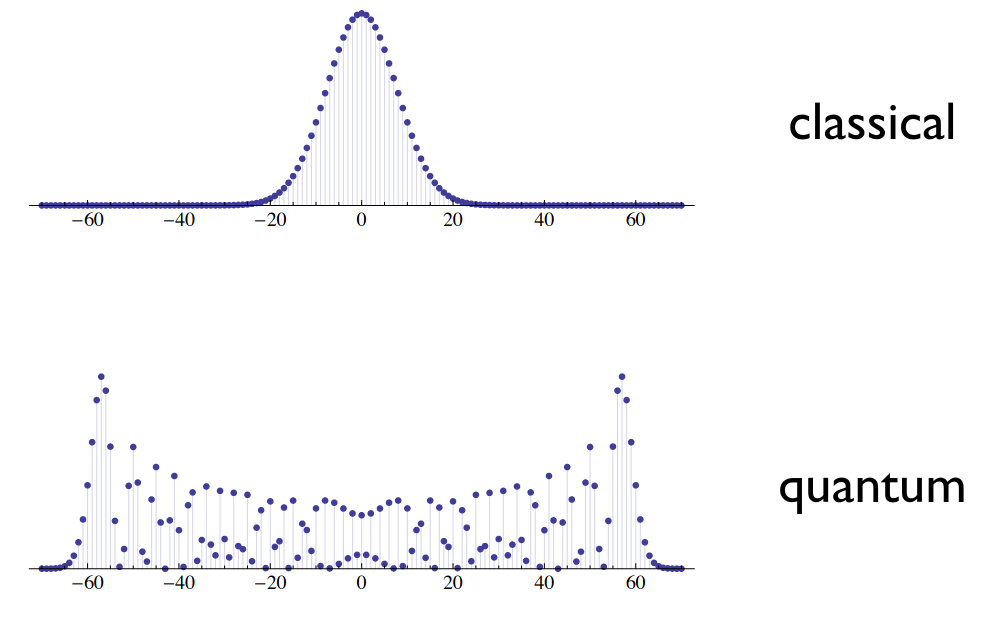
\includegraphics[width=60mm]{images/walks.png}
    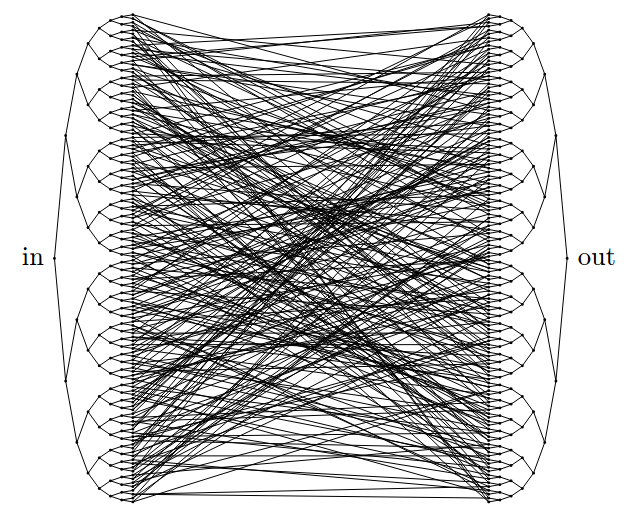
\includegraphics[width=50mm]{images/walks2.png}
    \caption{Quantum vs Classical Random Walks}
    % \label{fig:my_label}
\end{figure}

There are two kinds of quantum walks: discrete and continuous quantum walks. The main difference between these two sets is the timing used to apply corresponding evolution operators.
\begin{itemize}
\item \textbf{Discrete Quantum Walks}: It consists of two quantum mechanical systems, named a walker and a coin (for random element selection), as well as an evolution operator which is applied to both systems only in discrete time steps. The mathematical structure of this model is evolution via unitary operator, i.e. $\ket\psi_{t_2}=\hat{U}\ket\psi_{t_1}$
\item \textbf{Continuous Quantum Walks}: consists of a walker and
an evolution (Hamiltonian) operator of the system that can be applied with no timing restrictions at all, i.e. the walker walks any time. The mathematical structure of this model is evolution via the Schr\"{o}dinger equation, i.e. $\ket\psi_t=e^{-\frac{iHt}{\hbar}}\ket\psi_0$
\end{itemize}

\subsubsection{Defining a Discrete Quantum Walk on a Graph}

Let $G=(V,E)$ be a $d-$regular graph with $\abs{V}$=n, and $\mathcal{H}_v$ be the Hilbert space spanned by states $\ket v$ where $v\in V$. We also define $\mathcal{H}_A$, which is the coin space, as an auxiliary Hilbert space of dimension $d$ spanned by the basis state $\{\ket i|i\in\{1,\ldots,d\}\}$, and $\hat{C}$, which is the coin operator and a unitary transformation on $\mathcal{H}_A$. We also define a shift operator $\hat{S}$ on $\mathcal{H}_v\otimes\mathcal{H}_A$ such that $\hat{S}\ket{a,v}=\ket{a,u}$ where $u$ is the $a^{\text{th}}$ neighbour of $v$.

Finally we define one step of the quantum walk on $G$ as $\hat{U}=\hat{S}\left(\hat{C}\otimes\hat{I}\right)$. And if the quantum walk starts with an initial state $\ket\psi_0$, then the state after $t$ steps can be expressed as $\ket\psi_t=\hat{U}^t\ket\psi_0$

\subsubsection{Defining a Continuous Quantum Walk on a Graph}

Let $G=(V,E)$ be a graph with $\abs{V}$=n. We first define a generator matrix $M$ of order $n$ given by
$$M_{ab}=\begin{cases}
-\gamma,&a\ne b,(a,b)\in G\\
0,&a\ne b,(a,b)\notin G\\
k\gamma,&a=b\text{ and }k\text{ is the degree of vertex }a\text{ in }G
\end{cases}
$$
Now we define a Hamiltonian $\hat{H}$ with elements from matrix $M$ in a Hilbert space $\mathcal{H}$ with basis $\{\ket1,\ket2,\ldots,\ket n\}$. That is,
$$\left<a|\hat{H}|b\right>=M_{ab}$$

Now for a quantum walk starting in initial state $\ket\psi_0$, then the state after time $t$ can be expressed as
$$\ket\psi_t=e^{-i\hat{H}t}\ket\psi_0$$

\subsection{Szegedy Quantum Walk}
Szegedy defined a discrete-time quantum walk corresponding to an arbitrary discrete-time classical Markov chain in \cite{1366222}. Based on his work, Andrew Childs described a discrete-time quantum walk corresponding to a general $N\times N$ Hermitian matrix $H$.\newline

First, Childs fixed an orthonormal basis $\{\ket j:j=1,2,\ldots,N\}$ of $\mathbb{C}^N$, and
$$\text{abs}(H)=\sum_{j,k=1}^N\abs{H_{jk}}\ket j\bra k$$\label{abs_def}
is the elementwise absolute value of $H$. Now we define the principal eigenvector of $\text{abs}(H)$, i.e., the eigenvector with eigenvalue $||\text{abs}(H)||$ to be
$$\ket d=\sum_{j=1}^Nd_j\ket j$$
Now Childs defines $N$ orthonormal quantum states $\ket{\psi_1},\ldots,\ket{\psi_N}\in\mathbb{C}^N\times\mathbb{C}^N$ as
$$\ket{\psi_j}=\frac{1}{\sqrt{||\text{abs}(H)||}}\sum_{k=1}^N\sqrt{H_{jk}^*\frac{d_k}{d_j}}\ket{j,k}$$\label{szegedy_quantum_states}
where the state $\ket{\psi_j}$ is similar to a state $\ket j\otimes\ket{\phi_j}$ if $H$ represented a graph with nodes $\{\ket1,\ldots,\ket N\}$ and $\ket{\phi_k}=\sum_{k=1}^Na_k\ket k$ is the superposition of all the neighbours of $\ket j$ and $a_k$ is the amplitude corresponding to the  edge weight of the edge $(j,k)$ (as $H_{jk}$ corresponds to the edge weight in an adjancency matrix).

\subsubsection{Swap Operator}
The function of the swap operator $S$ is
$$S\ket{j,k}=\ket{k,j}$$
Thus, $S=S^{\dagger}$ and $SS^{\dagger}=S^2=\mathbb{I}$.

\subsubsection{Discrete Time Quantum Walk}
Childs defines the discrete-time quantum walk (Szegedy) corresponding to $H$ as the unitary operator obtained
by first reflecting about $\text{span}\{\ket{\psi_j}\}$ and then exchanging the two registers with the swap operator $S$. To formally define this, we first define the isometry mapping from $\ket j\in\mathbb{C}^N$ to $\ket{\psi_j}\in\mathbb{C}^N\times\mathbb{C}^N$ as
$$T=\sum_{j=1}^N\ket{\psi_j}\bra j$$\label{T_def}
Then $TT^{\dagger}$ is the projector onto $\text{span}\{\ket{\psi_j}\}$. And thus the walk operator is defined as $U=iS(2TT^{\dagger}-\mathbb{I})$\label{szegedy_walk_operator}. Now we consider the eigenvalues and eigenvectors for $\frac{H}{||\text{abs}(H)||}\ket\lambda$,
$$\frac{H}{||\text{abs}(H)||}\ket\lambda=\lambda\ket\lambda$$
We get the eigenvalues and eigenvectors of the walk operator $U$ to be
$$\ket{\mu_{\pm}}=\frac{\mathbb{I}-e^{\pm i\arccos\lambda}S}{\sqrt{2(1-\lambda^2)}}T\ket\lambda,\mu_{\pm}=\pm e^{\pm i\arcsin\lambda}$$\label{eigenvalue_eigenvector_szegedy_walk_operator_def}

\section{Hamiltonian Simulation using Quantum Walk}

No-fast-forwarding theorem states that the optimal number of steps required to simulate an evolution for time $t$ is linear in $t$. This can be done using Szegedy Quantum Walks and phase estimation.

Before moving on to the procedure for Hamiltonian simulation, we observe that for any state $\ket\psi\in\mathbb{C}^N\times\mathbb{C}^N$, we can write $T\ket\psi$ as
\begin{align*}
T\ket\psi&=\sum_\lambda \psi_\lambda T\ket\lambda\\
&=\sum_\lambda \psi_\lambda\left(\frac{1-\lambda e^{-i\arccos\lambda}}{\sqrt{2(1-\lambda^2)}}\ket{\mu_+}+\frac{1-\lambda e^{i\arccos\lambda}}{\sqrt{2(1-\lambda^2)}}\ket{\mu_-}\right)
\end{align*}

To simulate $H$ using the corresponding discrete-time quantum walk operator $U$ a phase of $e^{i\lambda t}$ is to be introduced for the $\lambda$ term of the superposition observed in the above expression. The procedure used for simulation is:
\begin{enumerate}
\item Apply $T$ to the input state $\ket\psi$
\item Perform phase estimation of $U$, estimating a phase $\pm e^{\pm i\arcsin\lambda}$ for the component $T\ket\lambda$
\item Use estimate of $\arcsin\lambda$ to get estimate of $\lambda$, $\Tilde{\lambda}$.
\item Induce the phase $e^{-i\Tilde{\lambda}t}$ and uncompute $\Tilde{\lambda}$ by performing phase estimation in reverse.
\item Finally apply reverse isometry $T^{\dagger}$
\end{enumerate}

Now for an eigenstate-eigenvalue pair $\ket\theta,e^{i\theta}$ of the discrete-time quantum walk, let $P$ denote the isometry that performs phase estimation on this walk. Then $P$ can be defined as follows
$$P\ket\theta=\sum_\phi a_{\phi|\theta}\ket{\theta,\phi}$$\label{P_def}
where $a_{\phi|\theta}$ is the amplitude for the estimate $\phi$. And let $F_t$ be the unitary operation that applies the desired phase to a given value-estimate state. That is,
$$F_t\ket{\theta,\phi}=e^{-it\sin\phi}\ket{\theta,\phi}$$\label{Ft_def}

Childs claims that the simulation of Hamiltonian evolution $e^{iHt}$ is $T^{\dagger}P^{\dagger}F_tPT$. To prove this claim, Child derived the inner product between the expected evolved state, $e^{-iHt}\ket\psi$, and the simulated evolved state, $T^{\dagger}P^{\dagger}F_tPT\ket\psi$ to be
$$\left<\psi|e^{iHt}T^{\dagger}P^{\dagger}F_tPT|\psi\right>=\sum_{\lambda,\phi}\abs{\psi_\lambda}^2e^{i(\lambda-\sin\phi)t}\frac{\abs{a_{\phi|\arcsin\lambda}}^2+\abs{a_{\phi|\pi-\arcsin\lambda}}^2}{2}
$$
He then went on to derive lower bound for the fidelity of this simulation to be
$$\abs{\left<\psi|e^{iHt}T^{\dagger}P^{\dagger}F_tPT|\psi\right>}\geq1 - \frac{t^2}{2}\min_{\theta \in [0, 2\pi)} \sum_\phi (\theta - \phi)^2 |a_{\phi|\theta}|^2$$

To further quantify the fidelity of the simulation, evaluation of performance of phase estimation is required. In standard phase
estimation modulo $M$, we begin from the state of equal superposition, that is $\frac{1}{\sqrt M}\sum_{x=0}^{M-1}\ket x$. Although there are some other states that, starting from whom give better results. One particular state that Childs mentioned is
$$\sqrt{\frac{2}{M+1}}\sum_{x=0}^{M-1}\sin\left(\frac{\pi(x+1)}{M+1}\right)\ket x$$
He claims, and goes on to prove that this initial state minimizes the variance of the estimate and gives the best bound for the fidelity of the simulation.\newline

\label{assumptions}The probability distribution of estimates of $\theta$ with this initial state is
$$\abs{a_{\theta+\Delta|\theta}}^2=\frac{\cos^2\left(\Delta\frac{M+1}{2}\right)\sin^2\left(\frac{\pi}{M+1}\right)}{2M(M+1)\sin^2\left(\frac{\Delta}{2}+\frac{\pi}{2(M+1)}\right)\sin^2\left(\frac{\Delta}{2}-\frac{\pi}{2(M+1)}\right)}$$
where the estimated phase is $\frac{2\pi j}{M}=\theta+\Delta$ for some integer $j$. A range of angles can be chosen such that $\Delta=\Delta_0+\frac{2\pi j}{M}$, where $0\leq\Delta_0\leq\frac{2\pi}{M}$ and $-\lceil \frac{M}{2}\rceil+1\leq j\leq\lfloor\frac{M}{2}\rfloor$.\newline

With these assumptions, and for sufficiently large $M$, we get that the bound on the fidelity of the simulation is atleast $1 - 93t^2/M^2$. Thus we find that $M = O(t/\sqrt \delta)$ steps suffice to obtain fidelity at least $1-\delta$. Hence, the gate complexity of simulation is also
$$O(t/\sqrt \delta)$$

With $K$ applications of the operator $U$ for phase estimation of $\arcsin\lambda$, the variance is approximately $\left(\frac{\pi}{K}\right)^2$, which means the variance in estimate of $\lambda$ is $O\left(\frac{||H||_1^2}{\eps^2K^2}\right)$ and that translates to error being $O\left(\frac{||H||_1t}{\eps K}\right)$. Taking $\eps=1$, to achieve atleast $1-\delta$ fidelity, $K=O\left(\frac{||H||_1t}{\sqrt\delta}\right)$. Hence, the query complexity of simulation is
$$O\left(\frac{d||H||_{max}t}{\sqrt\delta}\right)$$
\textit{Note that $||H||_1\le d||H||_{max}$ as the Hamiltonian is given to be d-sparse. Also, we use this upper bound for complexity as $||H||_1$ is often unknown.}

% \section{Example Implementation}
% We will explain the quantum walk approach using a toy Hamiltonian during the presentation. The explanation will also be added here while submitting the final draft.
% \newline

% \begin{center} \textcolor{red}{\textbf{TODO}} \end{center}

\section{Qubitization}
Qubitization provides us with a general framework to understand a high-dimensional space as the direct sum of a large number of $2$-dimensional spaces on which we act simultaneously and without their interfering with each other.\newline

Qubitization is found to perform better than older Hamiltonian simulation techniques for most cases. But, its use cases are not constrained to the simulation of Hamiltonians. It can be applied to understand and discover new algorithms and properties especially in the field of quantum walks.

\subsection{Description}
Before we delve into qubitization, we should note that in quantum computing, embedding in a $2$-dimensional space is not computationally expensive. A single auxiliary qubit is enough to double the dimension of the vector space used to represent the quantum information being processed. This is way treating qubits classically results in dealing with exponential space since we require a vector space of dimension $2^n$ to represent a quantum state defined by $n$ qubits.\newline

\subsubsection{About the routine}
\begin{itemize}
    \item Qubitization is based on the block encoding technique.
    \begin{figure}[H]
        \centering
        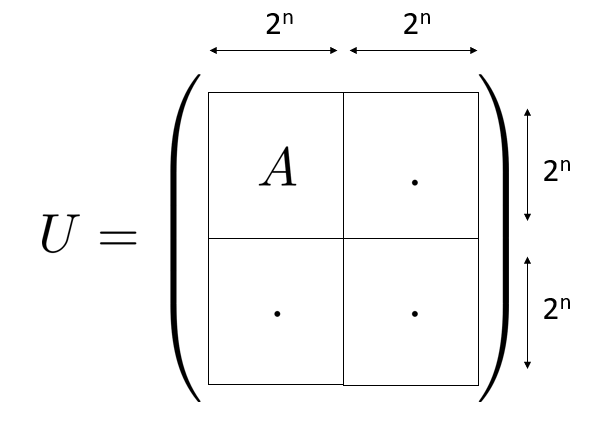
\includegraphics[width=40mm]{images/encoding.png}
        % \caption{Caption}
        % \label{fig:my_label}
    \end{figure}
    \item It relies on the decomposition of the $2^{n + 1}$ dimensional space on which $U$ acts into $2^n$ spaces, each of dimension $2$.
    \item Each such space of dimension $2$ is generated by an eigenvector of $A$ and another associated vector.
    \item Thus, qubitization refers to this decomposition in spaces of dimension $2$.
    \item Each eigenspace of $A$ is immersed in a space of dimension $2$, i.e. in the qubit space.
    \item Let $\Tilde{U}$ be the result of qubitizing $U$.
    $$\Tilde{U} = \oplus_{\lambda \in \Lambda(A)} W_{\text{qubit}, \lambda}$$
    Thus, $\Tilde{U}$ acts as the direct sum of ${2^n}$ unitary matrices of dimension $2$. We have one unitary of dimension $2$ per eigenvalue of $A$.
    \item For the purpose of Hamiltonian simulation, $A$ will be some Hamiltonian, $H$.
    \item $W_{\text{qubit}, \lambda}$ is a $2 \times 2$ diagonalizable unit matrix. Hence, $\forall\ {\lambda_W \in \Lambda(W)},\ |\lambda_W| = 1$. Furthermore, $\lambda_W$s are determined by $\lambda \in \Lambda(H)$. $W$ is referred to as the walk operator.
    $$W_{\text{qubit}, \lambda} \approx \begin{bmatrix}e^{i\cos^{-1}\lambda} & 0\\ 0 & e^{-i\cos^{-1}\lambda}\end{bmatrix}$$
    \item Now, the next step involves transforming the eigenvalues of the walk operator from $e^{\pm i\cos^{−1}\lambda}$ to $e^{−i\lambda t}$.
    \item This above transformation is possible by using any QSVT method (in the given diagram, we can see that QSP has been used).
    \item This method is suitable for finding static quantities such as the ground state of the associated $H$ (Hamiltonian). 
    \item For estimating ground state, we can just apply QPE directly to $W$.
\end{itemize}
\begin{figure}[H]
    \centering
    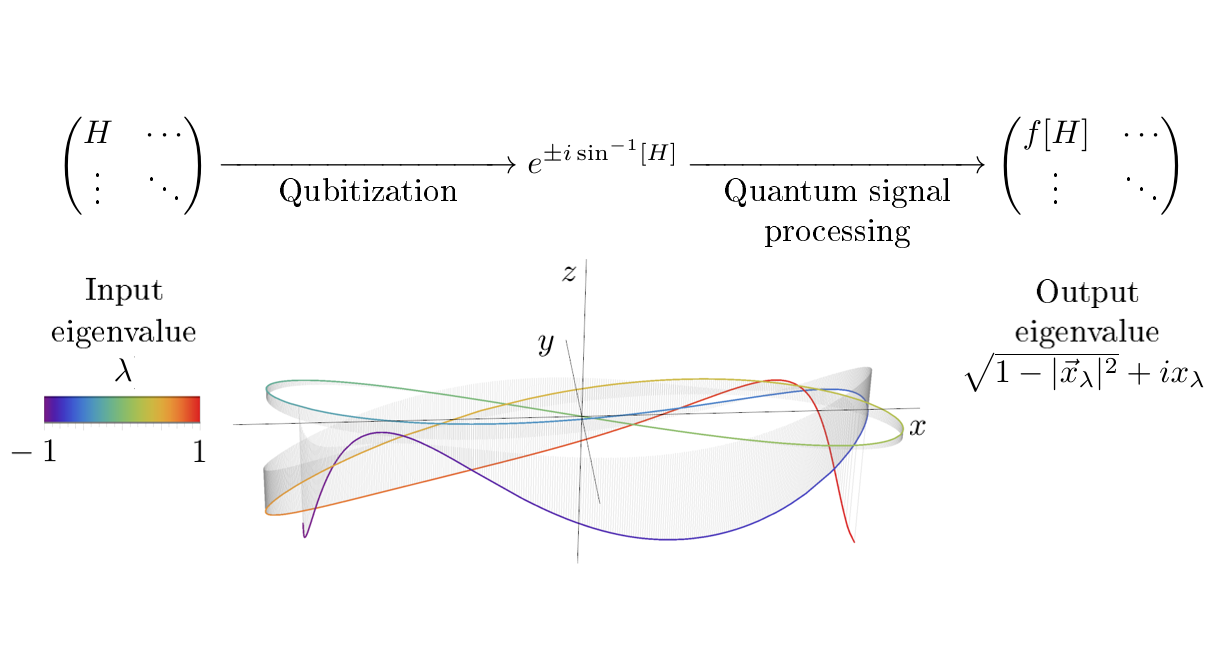
\includegraphics[width=100mm]{images/qubitization.png}
\end{figure}

\subsection{Wow qubitization rocks! Right? ... umm it does right?}
Now that we have a vague idea of how to go about implementing qubitization, it is worth noting that we require a few ($2$) subroutines (namely SELECT and PREPARE) to serve as interfaces for the Hamiltonian.\newline

Now unlike as in Trotterization, these subroutines are quantum in nature (and not classical). Thus, they require ancilla qubits (to be exact, logarithmically more qubits when compared to Trotterization) and hence might be infeasible for useful implementations in extremely near term NISQ-era. This same problems persists, to some extent, in the case of "Truncated Taylor Series" method and "Szegedy Quantum Walk", as well.\newline

However that said, qubitization is way better in simulating chemistry problems where there do not exist any self evident symmetries that can be taken advantage of.

\subsection{Implementation}
Let $H = \sum_j h_jH_j$ for unitary and Hermitian $H_j$ and $h_j \geq 0$. Thus, we need to implement $W = e^{\pm i \cos^{-1} (H/|h|_1)}$ where $|h|_1 = \sum_j |h_j|$.\newline

Now, consider the following subroutines:
\begin{itemize}
    \item \textbf{Reflection}: We have $\operatorname{SELECT} \ket{j} \ket{\psi} = \ket{j} H_j \ket{\psi}$.
    Now, $\operatorname{SELECT}^2\ket{j} \ket{\psi} = \ket{j} \ket{\psi}$ and the operator has eigenvalues $\pm 1$.
    \item Purpose of $\operatorname{SELECT}$ is to be able to access each of the $H_j$s.
    \item Now, we shall define the operator $\operatorname{PREPARE}$ to access the coefficients $h_j$s. 
    $$ \operatorname{PREPARE}\ket{0} = \sum_j \sqrt{\frac{h_j}{|h|_1}}\ket{j}$$
    \item Let us define $\mathcal{M}$ as follows.
    $$ \mathcal{M}\ket{0}^{\otimes n} = \begin{cases} -\ket{x} & \text{if } x = 0 \\ \ket{x} & \text{otherwise} \end{cases}$$
    \item Thus, $\mathcal{M}$ is a multiply controlled phase gate.
    \item \textbf{Another reflection}: $R = 1 - 2\operatorname{PREPARE} \ket{0}\bra{0} \operatorname{PREPARE}^{\dagger}$.
    \item Thus, we have $R = \operatorname{PREPARE} (\mathcal{M}) \operatorname{PREPARE}^{\dagger}$
\end{itemize}
Thus, the walk operatoor can be implemented as $W = \operatorname{(SELECT)}\ (R)$ which again can be seen to implement an operator that is equivalent (up to an isometry) to $e^{\pm i \cos^{-1}(H/|h|_1)}$.

% \section{Simulating non-sparse Hamiltonians}
% If a Hamiltonian is not sparse then, we cannot jot down the nonzero entries of a row in polynomial time - hence it will no longer be efficiently row computable. However, if the Hamiltonian gas a 

\nocite{*}
\bibliographystyle{unsrt}
\bibliography{references}

\newpage
\appendix

% \chapter{Appendix}

\section{Quantum Walks}

\begin{theorem}\label{szegedy_quantum_states_orthonormal}
The quantum states defined by Childs in \ref{szegedy_quantum_states} $\ket{\psi_1},\ldots,\ket{\psi_N}$ are orthonormal.
\end{theorem}
\begin{proof}
$$\braket{\psi_j}{\psi_k}=\frac{1}{||\text{abs}(H)||}\sum_{l_1,l_2=1}^N\sqrt{H_{jl_1}H_{kl_2}^*\frac{d_{l_1}d_{l_2}}{d_jd_k}}\braket{j,l_1}{k,l_2}$$
Thus, it is clear that $\braket{\psi_j}{\psi_k}=0$ when $j\ne k$, that is the quantum states are orthogonal.
\begin{align*}
\centering
\braket{\psi_j}{\psi_j}&=\frac{1}{||\text{abs}(H)||}\sum_{k_1,k_2=1}^N\sqrt{H_{jk_1}H_{jk_2}^*\frac{d_{k_1}d_{k_2}}{d_j^2}}\braket{j,k_1}{j,k_2}\\
&=\frac{1}{||\text{abs}(H)||}\sum_{k=1}^N\abs{H_{jk}}\frac{d_k}{d_j}\\
&=1,\ \ \ \text{since }\text{abs}(H)\ket d=||\text{abs}(H)||\ket d
\end{align*}
Hence, the quantum states are orthonormal.
\end{proof}

\begin{theorem}\label{eigenvalue_eigenvector_szegedy_walk_operator}
Suppose that for the Hamiltonian to be simulated $H$, with $\text{abs}(H)$ defined in \ref{abs_def}, $\frac{H}{||\text{abs}(H)||}\ket\lambda=\lambda\ket\lambda$. Then the szegedy walk operator $U$ defined in \ref{szegedy_walk_operator} has two normalised eigenvectors
$$\ket{\mu_{\pm}}=\frac{\mathbb{I}-e^{\pm i\arccos\lambda}S}{\sqrt{2(1-\lambda^2)}}T\ket\lambda$$
with eigenvalues $\mu_{\pm}=\pm e^{\pm i\arcsin\lambda}$.
\end{theorem}
\begin{proof}
Considering the action of $U$ on the vector $T\ket\lambda$, we have
\begin{align*}
UT\ket\lambda&=iS(2TT^{\dagger}-\mathbb{I})T\ket\lambda\\
&=2iSTT^{\dagger}T\ket\lambda-iST\ket\lambda\\
&=iST\ket\lambda&(\text{since }T^{\dagger}T=\mathbb{I})
\end{align*}
Considering the effect of the swap operator on the inner product of two of our orthonormal states we get
\begin{align*}
\braket{\psi_j|S|\psi_k}&=\frac{1}{||\text{abs}(H)||}\sum_{l_1,l_2=1}^N\sqrt{H_{jl_1}H_{kl_2}^*\frac{d_{l_1}d_{l_2}}{d_jd_k}}\braket{j,l_1}{l_2,k}\\
&=\frac{H_{jk}}{||\text{abs}(H)||}
\end{align*}
Thus, we also get the following.
\begin{align*}
T^{\dagger}ST&=\sum_{j,k=1}^N\ket j\left<\psi_j|S|\psi_k\right>\bra k\\
&=\frac{H}{||\text{abs}(H)||}
\end{align*}
And now, we have:
\begin{align*}
UST\ket\lambda&=iS(2TT^{\dagger}-\mathbb{I})ST\ket\lambda\\
&=2iSTT^{\dagger}ST\ket\lambda-iS^2T\ket\lambda\\
&=2\lambda iST\ket\lambda-iT\ket\lambda
\end{align*}
The unnormalised eigenvector, let it be $\ket\mu$, is
\begin{align*}
\ket\mu&=\left(\mathbb{I}-e^{i\arccos\lambda}S\right)T\ket\lambda\\
&=\left(\mathbb{I}-ie^{i\arcsin\lambda}S\right)T\ket\lambda\\
&=T\ket\lambda+i\mu ST\ket\lambda
\end{align*}
Thus, we can now obtain an expression by equating $U\ket\mu=\mu\ket\mu$
\begin{align*}
U\ket\mu=\mu\ket\mu&\Longleftrightarrow UT\ket\lambda+i\mu UST\ket\lambda=\mu T\ket\lambda+i\mu^2ST\ket\lambda\\
&\Longleftrightarrow iST\ket\lambda+i\mu\left(2\lambda iST\ket\lambda-iT\ket\lambda\right)=\mu T\ket\lambda+i\mu^2ST\ket\lambda\\
&\Longleftrightarrow i(1+2i\lambda\mu)ST\ket\lambda=i\mu^2ST\ket\lambda\\
&\Longleftrightarrow \mu^2=1+2i\lambda\mu
\end{align*}
Thus, solving the quadratic equation obtained, we obtain the unnormalised eigenvalues
$$\mu=i\lambda\pm\sqrt{1-\lambda^2}=ie^{\arccos\lambda}=\pm e^{\arcsin\lambda}$$
And the normalisation factor is
\begin{align*}
\braket{\mu}{\mu}&=\left<\lambda|T^{\dagger}T|\lambda\right>+i\mu\left<\lambda|T^{\dagger}ST|\lambda\right>-i\mu^*\left<\lambda|T^{\dagger}S^{\dagger}T|\lambda\right>+\abs{\mu}^2\left<\lambda|T^{\dagger}S^{\dagger}ST|\lambda\right>\\
&=1+i\mu\lambda-i\mu^*\lambda+\abs{\mu}^2\\
&=2(1-\lambda^2),\ \ \ \text{since }\mu=i\lambda\pm\sqrt{1-\lambda^2}
\end{align*}

Hence, by combining these results we get our the expressions for eigenvalues and eigenvectors that we wanted to prove.
\end{proof}

\section{Hamiltonian simulation using quantum walk}

\begin{theorem}\label{T_lambda}
For the isometry mapping $T$ defined in \ref{T_def}, and for an eigenvector $\lambda$ of $\frac{H}{||\text{abs}(H)||}$
$$T\ket\lambda=\frac{1-\lambda e^{-i\arccos\lambda}}{\sqrt{2(1-\lambda^2)}}\ket{\mu_+}+\frac{1-\lambda e^{i\arccos\lambda}}{\sqrt{2(1-\lambda^2)}}\ket{\mu_-}$$
where $\mu_{\pm}$ and $\ket{\mu_{\pm}}$ are the eigenvalues and eigenvectors of the szegedy walk operator (\textit{ref \ref{eigenvalue_eigenvector_szegedy_walk_operator_def}})
\end{theorem}
\begin{proof}
Let $x,y\in\mathbb{C}$ such that
$$T\ket\lambda=x\ket{\mu_+}+y\ket{\mu_-}$$
Then,
\begin{align*}
T\ket\lambda&=x\ket{\mu_+}+y\ket{\mu_-}\\
&=\frac{x+y}{\sqrt{2(1-\lambda^2)}}T\ket\lambda-\frac{xe^{i\arccos\lambda}+ye^{-i\arccos\lambda}}{\sqrt{2(1-\lambda^2)}}ST\ket\lambda
\end{align*}
Thus, we get a system of linear equations as follows.
$$x+y=\sqrt{2(1-\lambda^2)},xe^{i\arccos\lambda}+ye^{-i\arccos\lambda}=0$$
And we solve this system to get the coefficients to be
$$x=\frac{1-\lambda e^{-i\arccos\lambda}}{\sqrt{2(1-\lambda^2)}},y=\frac{1-\lambda e^{i\arccos\lambda}}{\sqrt{2(1-\lambda^2)}}$$
and from that, we finally get
$$T\ket\lambda=\frac{1-\lambda e^{-i\arccos\lambda}}{\sqrt{2(1-\lambda^2)}}\ket{\mu_+}+\frac{1-\lambda e^{i\arccos\lambda}}{\sqrt{2(1-\lambda^2)}}\ket{\mu_-}$$
\end{proof}

\begin{theorem}\label{inner_product_derivation}
For the isometric mappings $T$ and $P$ defined in \ref{T_def} and \ref{P_def} respectively and the unitary operation defined in \ref{Ft_}def
$$\left<\psi|e^{iHt}T^{\dagger}P^{\dagger}F_tPT|\psi\right>=\sum_{\lambda,\phi}\abs{\psi_\lambda}^2e^{i(\lambda-\sin\phi)t}\frac{\abs{a_{\phi|\arcsin\lambda}}^2+\abs{a_{\phi|\pi-\arcsin\lambda}}^2}{2}
$$
\end{theorem}
\begin{proof}
First, we derive
\begin{align*}
PTe^{-iHt}\ket\lambda&=PT\left(\sum_{\lambda'}e^{-i\lambda't}\ket{\lambda'}\bra{\lambda'}\right)\ket\lambda\\
&=e^{-i\lambda t}PT\ket\lambda\\
&=e^{-i\lambda t}P\left(\frac{1-\lambda e^{-i\arccos\lambda}}{\sqrt{2(1-\lambda^2)}}\ket{\mu_+}+\frac{1-\lambda e^{i\arccos\lambda}}{\sqrt{2(1-\lambda^2)}}\ket{\mu_-}\right)\\
&=e^{-i\lambda t}\sum_\phi\left(a_{\phi|\arcsin\lambda}\frac{1-\lambda e^{-i\arccos\lambda}}{\sqrt{2(1-\lambda^2)}}\ket{\mu_+,\phi}+\right.\\
&\qquad\qquad\qquad \left.a_{\phi|\pi-\arcsin\lambda}\frac{1-\lambda e^{i\arccos\lambda}}{\sqrt{2(1-\lambda^2)}}\ket{\mu_-,\phi}\right)\end{align*}
And thus,
\begin{multline*}
F_tPT\ket\lambda=\sum_\phi e^{-it\sin\phi}\left(a_{\phi|\arcsin\lambda}\frac{1-\lambda e^{-i\arccos\lambda}}{\sqrt{2(1-\lambda^2)}}\ket{\mu_+,\phi}+\right.\\
\left.a_{\phi|\pi-\arcsin\lambda}\frac{1-\lambda e^{i\arccos\lambda}}{\sqrt{2(1-\lambda^2)}}\ket{\mu_-,\phi}\right)
\end{multline*}

Using orthonormality of eigenstates (\ref{szegedy_quantum_states_orthonormal}), and the previous observation, we derive the required inner product to be
\begin{align*}
\left<\psi|e^{iHt}T^{\dagger}P^{\dagger}F_tPT|\psi\right>&=\sum_\lambda\abs{\psi_\lambda}^2\left<\lambda|e^{iHt}T^{\dagger}P^{\dagger}F_tPT|\lambda\right>\\
&=\sum_{\lambda,\phi}\abs{\psi_\lambda}^2e^{i(\lambda-\sin\phi)t}\left(\abs{a_{\phi|\arcsin\lambda}}^2\abs{\frac{1-\lambda e^{-i\arccos\lambda}}{\sqrt{2(1-\lambda^2)}}}^2+\right.\\
&\qquad\left.\abs{a_{\phi|\pi-\arcsin\lambda}}^2\abs{\frac{1-\lambda e^{i\arccos\lambda}}{\sqrt{2(1-\lambda^2)}}}^2\right)\ \ \ (\braket{\mu_+}{\mu_-}=0)\\
&=\sum_{\lambda,\phi}\abs{\psi_\lambda}^2e^{i(\lambda-\sin\phi)t}\frac{\abs{a_{\phi|\arcsin\lambda}}^2+\abs{a_{\phi|\pi-\arcsin\lambda}}^2}{2}
\end{align*}
\end{proof}

\begin{theorem}\label{fidelity_derivation}
For the expression derived for inner product between the expected and predicted states of simulating the Hamiltonian $H$ for time $t$ in \ref{inner_product_derivation}, derive that the fidelity of the simulation is lower bounded by
$$1 - \frac{t^2}{2}\min_{\theta \in [0, 2\pi)} \sum_\phi (\theta - \phi)^2 |a_{\phi|\theta}|^2$$
\end{theorem}
\begin{proof}
Fidelity of the simulation is $\abs{\left<\psi|e^{iHt}T^{\dagger}P^{\dagger}F_tPT|\psi\right>}$ and the first step at taking the lower bound is to minimise the value on one parameter of the summation.
\begin{align*}
\abs{\left<\psi|e^{iHt}T^{\dagger}P^{\dagger}F_tPT|\psi\right>}&\geq\min_\lambda\sum_\phi\cos((\lambda-\sin\phi)t)\frac{\abs{a_{\phi|\arcsin\lambda}}^2+\abs{a_{\phi|\pi-\arcsin\lambda}}^2}{2}\\
&\geq\min_{\theta\in[0,2\pi)}\sum_\phi\cos((\sin\theta-\sin\phi)t)\abs{a_{\phi|\theta}}^2\\
&\geq 1 - \min_{\theta \in [0,2\pi)} \frac{1}{2} \sum_{\phi} ((\sin \theta - \sin\phi)t)^2 |a_{\phi|\theta}|^2\\
&\geq 1 - \frac{t^2}{2}\min_{\theta \in [0, 2\pi)} \sum_\phi (\theta - \phi)^2 |a_{\phi|\theta}|^2
\end{align*}
$\text{and this holds because, } \abs{\sin\theta-\sin\phi}\leq\abs{\theta-\phi}$.
\end{proof}

\begin{theorem}\label{numerical_fidelity_bound}
With the assumptions made in \ref{assumptions}, the lower bound for the fidelity of the simulation is $1 - 93t^2/M^2$.
\end{theorem}
\begin{proof}
With the given assumptions, for sufficiently large $M$,
\begin{align*}
|a_{\theta + \Delta|\theta}|^2 &\leq \frac{\pi^2}{2M^4\sin^2\left(\frac{\Delta}{2} + \frac{\pi}{2(M + 1)}\right)\sin^2\left(\frac{\Delta}{2} - \frac{\pi}{2(M + 1)}\right)}\\
&\leq \frac{128\pi^2}{M^4\Delta^4\left(1 - \frac{\pi^2}{\Delta^2(M + 1)^2}\right)^2}\\
&\leq \frac{512\pi^2}{9M^4\Delta^4}
\end{align*}

Here, the last step assumes that $\Delta \geq 2\pi/M$. Now, since we have $2\pi j/M \leq \Delta \leq 2\pi(j + 1)/M$, the following holds.

\begin{align*}
\sum_{\phi} (\theta - \phi)^2 |a_{\phi|\theta}|^2 &\leq \frac{4\pi^2}{M^2} + 2 \sum_{j = 1}^{\infty}\frac{128(j + 1)^2}{9M^2j^2}\\
&= \frac{4\pi^2}{M^2} + \frac{256}{9M^2}\left(\frac{15\pi^2 + \pi^4 + 180\zeta(3)}{90}\right)\\
&\leq \frac{186}{M^2}
\end{align*}

Now considering the previously derived bound on fidelity of the simulation, we get the value to be
\begin{align*}
\abs{\left<\psi|e^{iHt}T^{\dagger}P^{\dagger}F_tPT|\psi\right>}&\geq1 - \frac{t^2}{2}\min_{\theta \in [0, 2\pi)} \sum_\phi (\theta - \phi)^2 |a_{\phi|\theta}|^2\\
&\geq 1-\frac{t^2}{2}\cdot\frac{186}{M^2}=1-\frac{93t^2}{M^2}
\end{align*}
\end{proof}

\section{Decomposition Lemma}
\begin{theorem}
Let $H$ be a $d$-sparse, row-computable Hamiltonian over $n$ qubits. It is possible to decompose $H$ into $H=\sum_{m=1}^{(d+1)^{2} n^{6}} H_{m}$ where each $H_{m}$ is:

\begin{itemize}
  \item A sparse, row-computable Hamiltonian over $n$ qubits, and,

  \item A $2 \times 2$ combinatorially block diagonal.

\end{itemize}
\end{theorem}

\begin{proof}
For the Hamiltonian $H$, we label each entry of the matrix $H_{i, j}$ for $i<j$ (upper diagonal entries) by a colour ${ }^{1}$. The colour of an entry $\operatorname{col}_{H}(i, j)$ is defined as the tuple $\left(k, i \bmod k, j \bmod k, r_{H}(i, j), c_{H}(i, j)\right)$ where
$$
k= \begin{cases}1 & \text { if } i=j \\ \text { The lowest integer where } i \neq j \bmod \text { for } 2 \leq k \leq n^{2} & \text { otherwise }\end{cases}
$$
and
$$
r_{H}(i, j)= \begin{cases}0 & \text { if } H_{i, j}=0 \\ \text { The index of } H_{i, j} \text { in the list of all } \\ \text { non-zero elements in the } i^{t h} \text { row of } \mathrm{H} & \text { otherwise. }\end{cases}
$$
The definition of $c_{H}(i, j)$ is the same as Equation (16) but now for columns as opposed to rows. For values of $i>j$ (lower diagonal entries), we define $\operatorname{col}_{H}(i, j)=\operatorname{col}_{H}(j, i)$. We define $H_{m}$ to contain all entries from $H$ that are a particular colour $m$. As each entry of $H_{m}$ has a single assigned colour, we can reconstruct $H$ by a summation over all colours $\left(H=\sum H_{m}\right)$. As $H$ is Hermitian and each $H_{m}$ is symmetric about the diagonal (from $\left.\operatorname{col}_{H}(i, j)=\operatorname{col}_{H}(j, i)\right)$, it follows that every $H_{m}$ is also Hermitian. Also as $H$ is row sparse and row computable, it follows that each $H_{m}$ also has these properties. From this, one can see that the first requirement of Lemma $2.4$ are satisfied.

\begin{figure}[H]
    \centering
    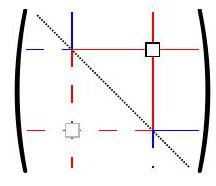
\includegraphics[width=40mm]{images/graph-matrix.jpg}
    \caption{How the colouring of the matrix restricts the possible structure of $H_{m}$}
    \label{fig:my_label}
\end{figure}

From the restraint of $r_{H}(i, j)$ and $c_{H}(i, j)$ on the colour tuple, we know that for a non-zero element of a matrix $H_{m}$ at position $(i, j)$, there are no other non-zero elements in row $i$ or column $j$ (red lines in upper half of Figure 1). Furthermore, the other tuple colouring components $(k, i \bmod k, j \bmod k)$ create the case where there exists only a single non-zero element of $H_{m}$ in the row $j$ or column $i$ in the position $(j, i)$ (blue lines in upper half of Figure 1). This case is reflected for $i<j$ as $\operatorname{col}_{H}(i, j)=\operatorname{col}_{H}(j, i)$ (dashed lines in Figure 1). From these two conditions, it leads that each matrix $H_{m}$ can be permuted to become a $2 \times 2$ block diagonal matrix where each mirror diagonal pair $\left(H_{i, j}\right.$, $H_{j, i}$ ) forms a block. Therefore each $H_{m}$ is a combinatorially block diagonal, proving the second part of the theorem.
\end{proof}

\begin{figure}[H]
    \centering
    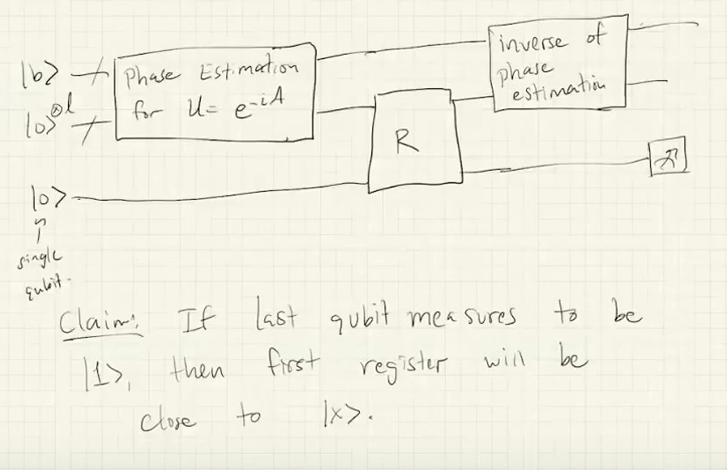
\includegraphics[width=\linewidth]{images/use case1.png}
    % \caption{C}
    % \label{fig:my_label}
\end{figure}

\begin{figure}[H]
    \centering
    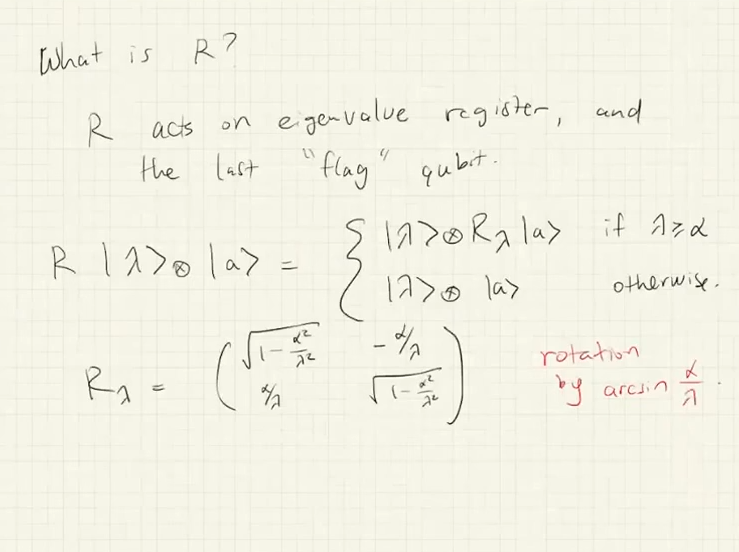
\includegraphics[width=\linewidth]{images/usecase2.png}
    % \caption{C}
    % \label{fig:my_label}
\end{figure}

\begin{figure}[H]
    \centering
    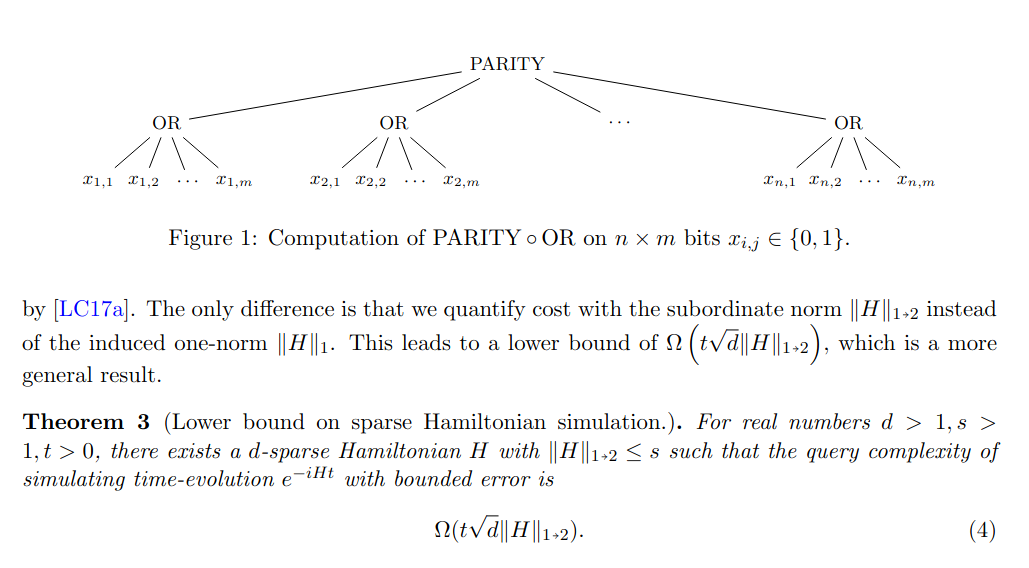
\includegraphics[width=\linewidth]{1.png}
    \caption{Caption}
    \label{fig:my_label}
\end{figure}

\begin{figure}[H]
    \centering
    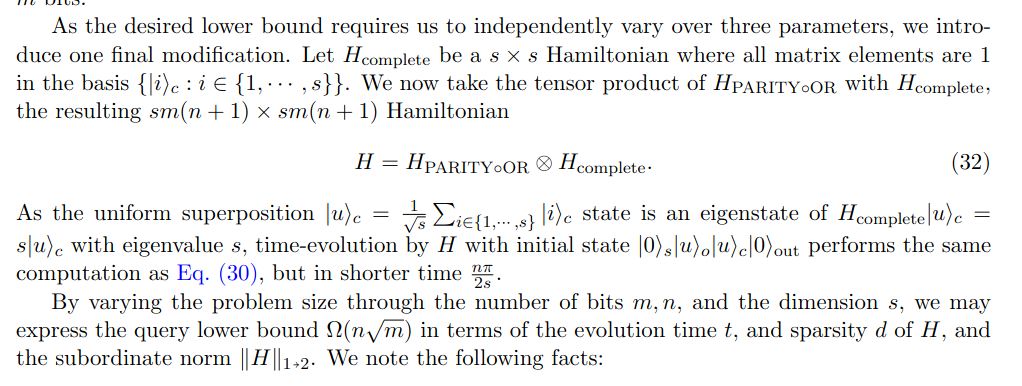
\includegraphics[width=\linewidth]{2.png}
    \caption{Caption}
    \label{fig:my_label}
\end{figure}

\begin{figure}[H]
    \centering
    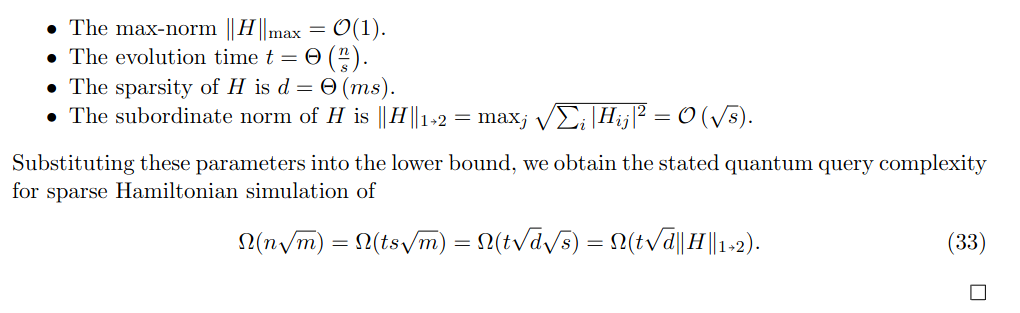
\includegraphics[width=\linewidth]{3.png}
    \caption{Caption}
    \label{fig:my_label}
\end{figure}

\end{document}